\documentclass[11pt,a4paper]{article}

% Packages
\usepackage[margin=2.5cm]{geometry}
\usepackage{microtype}
\usepackage{graphicx}
\usepackage{tikz}
\usetikzlibrary{shapes,arrows.meta,positioning,calc,fit,backgrounds,shadows.blur,decorations.pathmorphing,decorations.pathreplacing}
\usepackage{colortbl}
\usepackage{enumitem}
\usepackage{booktabs}
\usepackage{longtable}
\usepackage{hyperref}
\usepackage{xcolor}
\usepackage{fancyhdr}
\usepackage{titlesec}
\usepackage[most]{tcolorbox}
\usepackage{multicol}
\usepackage{amsmath,amssymb}
\usepackage{multirow}
\usepackage{setspace}
\usepackage{fontawesome5}
\usepackage{listings}

% Spacing
\setlength{\parskip}{3pt plus 1pt minus 1pt}
\setlength{\parindent}{0pt}

% Colors
\definecolor{primary}{HTML}{1A5276}
\definecolor{secondary}{HTML}{2E86C1}
\definecolor{accent}{HTML}{E74C3C}
\definecolor{lightbg}{HTML}{EBF5FB}
\definecolor{defbg}{HTML}{FDF2E9}
\definecolor{greenhl}{HTML}{27AE60}
\definecolor{purplehl}{HTML}{8E44AD}
\definecolor{codebg}{HTML}{F4F6F7}

% Hyperref
\hypersetup{colorlinks=true, linkcolor=primary, urlcolor=secondary, citecolor=primary}

% Code listings style
\lstset{
  backgroundcolor=\color{codebg},
  basicstyle=\ttfamily\small,
  keywordstyle=\color{primary}\bfseries,
  stringstyle=\color{greenhl},
  commentstyle=\color{gray},
  breaklines=true,
  frame=l,
  framerule=2pt,
  rulecolor=\color{secondary!40},
  xleftmargin=8pt,
  framexleftmargin=6pt,
  aboveskip=6pt,
  belowskip=6pt,
  showstringspaces=false,
  language=Python
}

% Header/Footer
\pagestyle{fancy}
\fancyhf{}
\fancyhead[L]{\small\textcolor{primary}{\textbf{Deep Learning --- Fundamentals Made Easy}}}
\fancyhead[R]{\small\textcolor{primary}{Lecture Handout}}
\fancyfoot[C]{\small\thepage}
\renewcommand{\headrulewidth}{0.5pt}
\renewcommand{\footrulewidth}{0.3pt}

% Section formatting
\titleformat{\section}{\Large\bfseries\color{primary}}{\thesection}{0.6em}{}[\vspace{2pt}\titlerule]
\titleformat{\subsection}{\large\bfseries\color{secondary}}{\thesubsection}{0.5em}{}
\titleformat{\subsubsection}{\normalsize\bfseries\color{primary}}{\thesubsubsection}{0.5em}{}
\titlespacing*{\section}{0pt}{14pt}{8pt}
\titlespacing*{\subsection}{0pt}{10pt}{5pt}

% Custom boxes
\newtcolorbox{definitionbox}[1][]{
  enhanced, breakable,
  colback=defbg, colframe=orange!60!black,
  colbacktitle=orange!70!black, coltitle=white,
  title={\faIcon{book}~#1}, fonttitle=\bfseries,
  boxrule=0pt, leftrule=4pt, arc=2pt,
  shadow={1mm}{-1mm}{0mm}{black!15},
  top=4pt, bottom=4pt, left=8pt, right=8pt
}
\newtcolorbox{conceptbox}[1][]{
  enhanced, breakable,
  colback=lightbg, colframe=secondary,
  colbacktitle=secondary, coltitle=white,
  title={\faIcon{lightbulb}~#1}, fonttitle=\bfseries,
  boxrule=0pt, leftrule=4pt, arc=2pt,
  shadow={1mm}{-1mm}{0mm}{black!15},
  top=4pt, bottom=4pt, left=8pt, right=8pt
}
\newtcolorbox{alertbox}[1][]{
  enhanced, breakable,
  colback=red!4, colframe=accent,
  colbacktitle=accent, coltitle=white,
  title={\faIcon{exclamation-triangle}~#1}, fonttitle=\bfseries,
  boxrule=0pt, leftrule=4pt, arc=2pt,
  shadow={1mm}{-1mm}{0mm}{black!12},
  top=3pt, bottom=3pt, left=8pt, right=8pt
}
\newtcolorbox{examplebox}[1][]{
  enhanced, breakable,
  colback=green!4, colframe=greenhl,
  colbacktitle=greenhl, coltitle=white,
  title={\faIcon{code}~#1}, fonttitle=\bfseries,
  boxrule=0pt, leftrule=4pt, arc=2pt,
  shadow={1mm}{-1mm}{0mm}{black!12},
  top=3pt, bottom=3pt, left=8pt, right=8pt
}

\begin{document}

% Title
\begin{center}
\vspace*{0.5cm}
{\Huge\bfseries\textcolor{primary}{Deep Learning}}\\[8pt]
{\Huge\bfseries\textcolor{primary}{Fundamentals Made Easy}}\\[16pt]
{\color{secondary}\rule{0.6\textwidth}{1.5pt}}\\[14pt]
{\Large\textsc{BSIT Data Science Lecture Handout}}\\[8pt]
{\large\textcolor{gray!70!black}{Concepts $\bullet$ Neural Networks $\bullet$ Architectures $\bullet$ Practical Examples}}
\vspace{0.3cm}
\end{center}

\tableofcontents
\newpage

%=============================================================
\section{Introduction to Deep Learning}
%=============================================================

\begin{definitionbox}[Deep Learning]
Deep learning is a branch of machine learning that uses \textbf{artificial neural networks with multiple layers} to learn patterns directly from data. It is especially powerful for complex data such as \textbf{images, text, speech, video, and large tabular datasets}.
\end{definitionbox}

\begin{conceptbox}[Simple Idea]
Think of deep learning as \textbf{stacking many small pattern detectors}. Early layers may learn simple patterns such as edges, colors, or short word sequences. Deeper layers combine those simple patterns into richer ideas such as objects in an image, sentiment in a sentence, or fraud patterns in transactions.
\end{conceptbox}

\subsection{Where Deep Learning Fits in AI}

\begin{center}
\begin{tikzpicture}[scale=1]
  \fill[black!8] (0.08,-0.08) circle (4.5cm);
  \fill[blue!6] (0,0) circle (4.5cm);
  \draw[thick, primary, line width=1.5pt] (0,0) circle (4.5cm);
  \node[font=\bfseries\large, primary] at (0,3.85) {\faIcon{robot}~Artificial Intelligence};
  \node[font=\scriptsize, primary!70, align=center] at (3.15,-3.2) {Search, planning,\\expert systems,\\recommendation};

  \fill[orange!8] (0,-0.4) circle (2.9cm);
  \draw[thick, orange!70!black, line width=1.2pt] (0,-0.4) circle (2.9cm);
  \node[font=\bfseries, orange!70!black] at (0,2.0) {\faIcon{brain}~Machine Learning};
  \node[font=\scriptsize, orange!50!black, align=center] at (-2.15,0.25) {Regression,\\classification,\\clustering};

  \fill[green!8] (0,-0.7) circle (1.5cm);
  \draw[thick, greenhl!70!black, line width=1.2pt] (0,-0.7) circle (1.5cm);
  \node[font=\bfseries\small, greenhl!70!black, align=center] at (0,-0.7) {\faIcon{project-diagram}\\Deep\\Learning};
\end{tikzpicture}
\end{center}

\begin{itemize}[leftmargin=1.5em, itemsep=3pt]
  \item \textbf{Artificial Intelligence (AI)} is the broad field of making machines behave intelligently.
  \item \textbf{Machine Learning (ML)} is a subset of AI that learns patterns from data.
  \item \textbf{Deep Learning (DL)} is a subset of ML that uses many-layer neural networks.
\end{itemize}

\subsection{Why Deep Learning Matters}

\begin{itemize}[leftmargin=*]
  \item It can learn useful features automatically instead of depending only on manual feature engineering.
  \item It performs very well when the data is large and complex.
  \item It powers modern systems such as face recognition, chatbots, translation, speech assistants, recommendation engines, and medical image analysis.
  \item It supports both predictive tasks and generative tasks such as text generation or image generation.
\end{itemize}

\subsection{When Deep Learning Is a Good Choice}

\begin{center}
\begin{tabular}{@{}p{6.2cm}p{6.2cm}@{}}
\toprule
\textbf{Deep Learning Often Fits Well} & \textbf{Traditional ML May Be Better First} \\
\midrule
Large image, audio, or text datasets & Small datasets with limited samples \\
Very complex relationships in the data & Problems where high interpretability is required \\
Tasks where automatic feature learning helps & Cases where a simple model already works well \\
Applications that can use GPU acceleration & Projects with very limited computing resources \\
\bottomrule
\end{tabular}
\end{center}

\begin{alertbox}[Important Note]
Deep learning is not always the best first model. In many business and classroom projects, a simpler method such as logistic regression, decision trees, or random forests may be easier to train, explain, and deploy.
\end{alertbox}

%=============================================================
\section{Neural Network Basics}
%=============================================================

\begin{definitionbox}[Artificial Neuron]
An artificial neuron receives inputs, gives each input a \textbf{weight}, adds a \textbf{bias}, and then applies an \textbf{activation function} to produce an output.
\[
z = w_1x_1 + w_2x_2 + w_3x_3 + b
\qquad
a = \text{activation}(z)
\]
This is one of the few formulas you need to remember. Everything else in deep learning is built by connecting many of these simple units together.
\end{definitionbox}

\subsection{Inside One Neuron}

\begin{center}
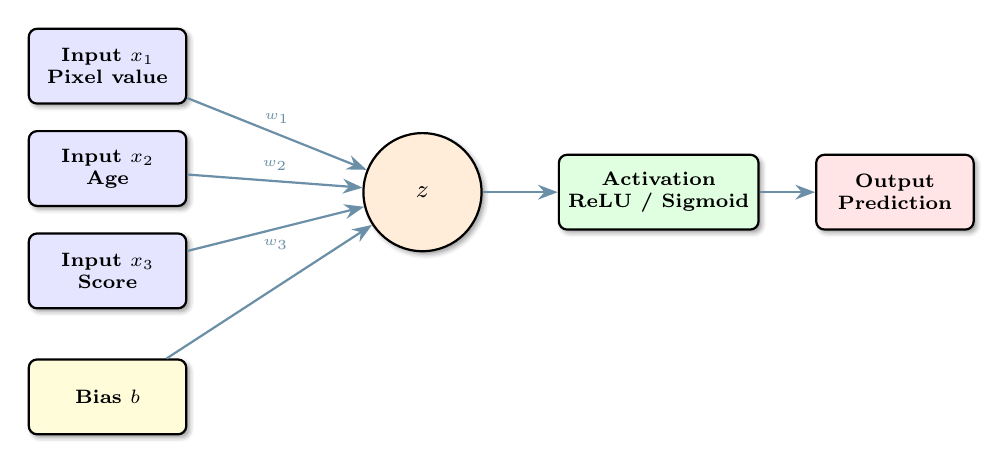
\begin{tikzpicture}[
  box/.style={rectangle, draw, thick, fill=#1, minimum width=2.0cm, minimum height=0.95cm, align=center, font=\scriptsize\bfseries, rounded corners=3pt,
    blur shadow={shadow blur steps=4, shadow xshift=0.4mm, shadow yshift=-0.4mm}},
  arr/.style={-{Stealth[length=2.5mm]}, thick, primary!65}
]
  \node[box=blue!10] (x1) at (0,2.2) {Input $x_1$\\Pixel value};
  \node[box=blue!10] (x2) at (0,0.9) {Input $x_2$\\Age};
  \node[box=blue!10] (x3) at (0,-0.4) {Input $x_3$\\Score};
  \node[box=yellow!15] (b) at (0,-2.0) {Bias $b$};

  \node[circle, draw, thick, fill=orange!15, minimum size=1.5cm, font=\small\bfseries,
    blur shadow={shadow blur steps=4, shadow xshift=0.4mm, shadow yshift=-0.4mm}] (sum) at (4,0.6) {$z$};
  \node[box=green!12] (act) at (7,0.6) {Activation\\ReLU / Sigmoid};
  \node[box=red!10] (out) at (10,0.6) {Output\\Prediction};

  \draw[arr] (x1) -- node[above, font=\tiny] {$w_1$} (sum);
  \draw[arr] (x2) -- node[above, font=\tiny] {$w_2$} (sum);
  \draw[arr] (x3) -- node[below, font=\tiny] {$w_3$} (sum);
  \draw[arr] (b) -- (sum);
  \draw[arr] (sum) -- (act);
  \draw[arr] (act) -- (out);
\end{tikzpicture}
\end{center}

\begin{itemize}[leftmargin=*]
  \item \textbf{Inputs} are the feature values.
  \item \textbf{Weights} tell the model how important each input is.
  \item \textbf{Bias} lets the neuron shift its output.
  \item \textbf{Activation} adds non-linearity so the network can learn complex patterns.
\end{itemize}

\subsection{Layers in a Neural Network}

\begin{center}
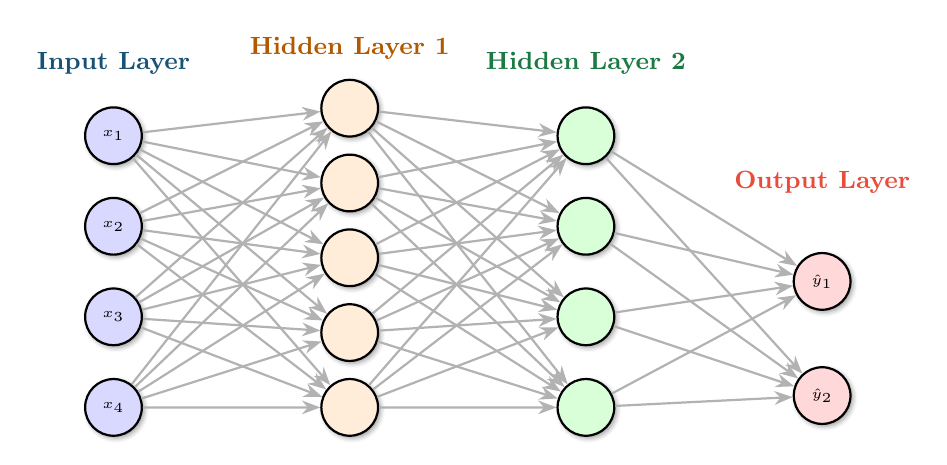
\begin{tikzpicture}[
  neuron/.style={circle, draw, thick, fill=#1, minimum size=0.72cm, font=\tiny\bfseries,
    blur shadow={shadow blur steps=4, shadow xshift=0.3mm, shadow yshift=-0.3mm}},
  arr/.style={-{Stealth}, thick, black!30}
]
  \foreach \i in {1,2,3,4} {
    \node[neuron=blue!15] (i\i) at (0, -\i*1.15+3) {$x_{\i}$};
  }
  \foreach \j in {1,2,3,4,5} {
    \node[neuron=orange!15] (h1\j) at (3, -\j*0.95+3.15) {};
  }
  \foreach \j in {1,2,3,4} {
    \node[neuron=green!15] (h2\j) at (6, -\j*1.15+3) {};
  }
  \foreach \k in {1,2} {
    \node[neuron=red!15] (o\k) at (9, -\k*1.45+1.45) {$\hat{y}_{\k}$};
  }

  \foreach \i in {1,2,3,4} {
    \foreach \j in {1,2,3,4,5} {
      \draw[arr] (i\i) -- (h1\j);
    }
  }
  \foreach \i in {1,2,3,4,5} {
    \foreach \j in {1,2,3,4} {
      \draw[arr] (h1\i) -- (h2\j);
    }
  }
  \foreach \i in {1,2,3,4} {
    \foreach \j in {1,2} {
      \draw[arr] (h2\i) -- (o\j);
    }
  }

  \node[font=\small\bfseries, primary, above] at (0, 2.5) {Input Layer};
  \node[font=\small\bfseries, orange!70!black, above] at (3, 2.7) {Hidden Layer 1};
  \node[font=\small\bfseries, greenhl!70!black, above] at (6, 2.5) {Hidden Layer 2};
  \node[font=\small\bfseries, accent, above] at (9, 1.0) {Output Layer};
\end{tikzpicture}
\end{center}

\begin{definitionbox}[Meaning of \textit{Deep}]
A neural network becomes \textbf{deep} when it has more than one hidden layer. More layers allow the model to learn more abstract patterns, but they also make training more challenging and computationally expensive.
\end{definitionbox}

\subsection{Common Activation Functions}

\rowcolors{2}{white}{defbg}
\begin{longtable}{@{}p{3cm}p{4cm}p{5.8cm}@{}}
\toprule
\rowcolor{primary!15}
\textbf{Activation} & \textbf{Main Idea} & \textbf{Typical Use} \\
\midrule
\endhead
ReLU & Keeps positive values, changes negative values to 0 & Most hidden layers in modern networks because it is simple and fast \\
\addlinespace
Sigmoid & Converts a value into a score between 0 and 1 & Binary classification output such as yes/no prediction \\
\addlinespace
Tanh & Produces values between $-1$ and $1$ & Sometimes used in recurrent networks \\
\addlinespace
Softmax & Converts several scores into probabilities that sum to 1 & Multi-class classification output such as digit 0 to 9 \\
\bottomrule
\end{longtable}

\begin{conceptbox}[Easy Memory Trick]
Use \textbf{ReLU} inside the network, \textbf{Sigmoid} for a binary output, and \textbf{Softmax} for a multi-class output.
\end{conceptbox}

%=============================================================
\section{How a Neural Network Learns}
%=============================================================

\subsection{Forward Pass}

\begin{definitionbox}[Forward Pass]
During the forward pass, the input data moves from the input layer through hidden layers to the output layer. The network produces a prediction such as a class label, a probability, or a numeric value.
\end{definitionbox}

\subsection{Loss Function}

\begin{conceptbox}[Loss = Prediction Error]
The loss function tells the model \textbf{how wrong it is}. If the prediction is close to the true answer, the loss is small. If the prediction is far from the true answer, the loss is large.
\end{conceptbox}

Typical examples:
\begin{itemize}[leftmargin=*]
  \item \textbf{Binary cross-entropy:} Used for yes/no classification.
  \item \textbf{Categorical cross-entropy:} Used for multi-class classification.
  \item \textbf{Mean squared error:} Used for regression.
\end{itemize}

\subsection{Backpropagation}

\begin{definitionbox}[Backpropagation]
Backpropagation is the process of sending the prediction error backward through the network so the weights can be adjusted. In simple words, it answers the question: \textit{Which weights caused the mistake, and how should they change?}
\end{definitionbox}

\begin{conceptbox}[Intuition]
Imagine a group project where the final answer is wrong. Backpropagation is like checking each team member's contribution to find who should change their part a little. The network does the same with its weights.
\end{conceptbox}

\subsection{Gradient Descent, Epochs, and Batches}

\begin{itemize}[leftmargin=*]
  \item \textbf{Gradient descent} updates weights to reduce the loss.
  \item \textbf{Learning rate} controls how big each update is.
  \item \textbf{Epoch} means one full pass through the training dataset.
  \item \textbf{Batch} means a smaller chunk of data used in one update step.
\end{itemize}

\begin{alertbox}[Why the Learning Rate Matters]
If the learning rate is too small, training is very slow. If it is too large, the model may jump around and fail to learn a stable solution.
\end{alertbox}

\subsection{The Training Cycle}

\begin{center}
\begin{tikzpicture}[
  step/.style={rectangle, draw, thick, fill=#1, minimum width=2.2cm, minimum height=1.05cm, align=center, font=\footnotesize\bfseries, rounded corners=4pt,
    blur shadow={shadow blur steps=5, shadow xshift=0.5mm, shadow yshift=-0.5mm}},
  arr/.style={-{Stealth[length=2.5mm]}, very thick, primary!60, line width=1.15pt}
]
  \node[step=blue!12] (s1) at (0,0) {\faIcon{database}\\Input Batch};
  \node[step=cyan!12] (s2) at (2.9,0) {\faIcon{project-diagram}\\Forward Pass};
  \node[step=orange!12] (s3) at (5.8,0) {\faIcon{exclamation-circle}\\Compute Loss};
  \node[step=green!12] (s4) at (8.7,0) {\faIcon{undo}\\Backpropagation};
  \node[step=red!10] (s5) at (11.6,0) {\faIcon{sliders-h}\\Update Weights};

  \draw[arr] (s1) -- (s2);
  \draw[arr] (s2) -- (s3);
  \draw[arr] (s3) -- (s4);
  \draw[arr] (s4) -- (s5);
  \draw[arr, dashed, secondary] (s5.south) to[bend right=35] node[below, font=\tiny\itshape, secondary] {repeat for many batches and epochs} (s1.south);
\end{tikzpicture}
\end{center}

\subsection{Important Hyperparameters}

\rowcolors{2}{white}{defbg}
\begin{longtable}{@{}p{3.4cm}p{9.9cm}@{}}
\toprule
\rowcolor{primary!15}
\textbf{Hyperparameter} & \textbf{What It Controls} \\
\midrule
\endhead
Learning rate & Size of each weight update during training \\
\addlinespace
Batch size & Number of training examples processed at one time \\
\addlinespace
Epochs & Number of full passes through the training data \\
\addlinespace
Number of layers & Depth of the network \\
\addlinespace
Number of neurons & Capacity of each layer to learn patterns \\
\addlinespace
Dropout rate & Fraction of neurons randomly ignored during training to reduce overfitting \\
\bottomrule
\end{longtable}

%=============================================================
\section{Key Terminology for Beginners}
%=============================================================

\rowcolors{2}{white}{defbg}
\begin{longtable}{@{}p{3.5cm}p{10cm}@{}}
\toprule
\rowcolor{primary!15}
\textbf{Term} & \textbf{Meaning} \\
\midrule
\endhead
Feature & An input value such as age, pixel intensity, or word index \\
\addlinespace
Weight & A learned value showing how strongly an input affects the output \\
\addlinespace
Bias & An extra learned value that shifts the neuron output \\
\addlinespace
Neuron & A small computational unit that transforms inputs into an output \\
\addlinespace
Layer & A group of neurons at the same stage in the network \\
\addlinespace
Activation function & A rule that transforms a neuron output into a usable signal \\
\addlinespace
Parameter & A value learned during training, such as a weight or bias \\
\addlinespace
Hyperparameter & A value chosen before training, such as learning rate or batch size \\
\addlinespace
Loss & A number showing how wrong the prediction is \\
\addlinespace
Optimizer & The method used to update weights, such as SGD or Adam \\
\addlinespace
Overfitting & When the model memorizes training data and performs poorly on new data \\
\addlinespace
Generalization & The ability to work well on unseen data \\
\bottomrule
\end{longtable}

%=============================================================
\section{Preparing Data for Deep Learning}
%=============================================================

\begin{conceptbox}[Garbage In, Garbage Out]
Even a powerful deep learning model cannot rescue poor data. Clean, relevant, and well-prepared data is still the foundation of good performance.
\end{conceptbox}

\subsection{How Different Data Types Are Prepared}

\rowcolors{2}{white}{defbg}
\begin{longtable}{@{}p{3cm}p{4cm}p{6.5cm}@{}}
\toprule
\rowcolor{primary!15}
\textbf{Data Type} & \textbf{Representation} & \textbf{Common Preparation Steps} \\
\midrule
\endhead
Images & Pixel grids & Resize, normalize pixel values, augment with flips or rotations \\
\addlinespace
Text & Tokens or embeddings & Clean text, tokenize, pad sequences, build embeddings \\
\addlinespace
Audio & Waveforms or spectrograms & Trim noise, convert to features, standardize length \\
\addlinespace
Tabular data & Rows and columns & Handle missing values, encode categories, scale numeric features \\
\bottomrule
\end{longtable}

\subsection{Train, Validation, and Test Sets}

\begin{definitionbox}[Data Splitting]
Split the dataset into:
\begin{itemize}[leftmargin=*]
  \item \textbf{Training set:} Used to learn the model.
  \item \textbf{Validation set:} Used to tune settings and monitor overfitting.
  \item \textbf{Test set:} Used only at the end for final evaluation.
\end{itemize}
For many classroom projects, a split such as \textbf{70\% training, 15\% validation, 15\% test} is a good starting point.
\end{definitionbox}

\subsection{Useful Preparation Techniques}

\begin{itemize}[leftmargin=*]
  \item Normalize or standardize numeric values.
  \item Encode text and categorical variables properly.
  \item Balance classes when one class is much rarer than the others.
  \item Use data augmentation for images to create more variety.
  \item Remove obvious noise, duplicates, and incorrect labels when possible.
\end{itemize}

\begin{alertbox}[A Common Beginner Mistake]
Never let the test set influence model design decisions. If you repeatedly tune the model using the test set, your final performance estimate becomes overly optimistic.
\end{alertbox}

%=============================================================
\section{Common Deep Learning Architectures}
%=============================================================

\rowcolors{2}{white}{defbg}
\begin{longtable}{@{}p{3cm}p{3.2cm}p{6.3cm}@{}}
\toprule
\rowcolor{primary!15}
\textbf{Architecture} & \textbf{Best For} & \textbf{Main Idea} \\
\midrule
\endhead
MLP (Multilayer Perceptron) & Tabular data, simple classification & Fully connected layers learn patterns from structured inputs \\
\addlinespace
CNN (Convolutional Neural Network) & Images and spatial data & Filters scan local regions and detect visual patterns such as edges and shapes \\
\addlinespace
RNN (Recurrent Neural Network) & Sequential data & The model remembers previous steps while processing the current step \\
\addlinespace
LSTM / GRU & Longer sequences and time series & Improved recurrent design that remembers useful information for longer \\
\addlinespace
Transformer & Text, language, vision, large AI systems & Attention lets the model focus on the most relevant parts of the input \\
\addlinespace
Autoencoder & Compression and anomaly detection & Learns how to encode input into a compact form and reconstruct it \\
\bottomrule
\end{longtable}

\subsection{A CNN Pipeline for Image Tasks}

\begin{center}
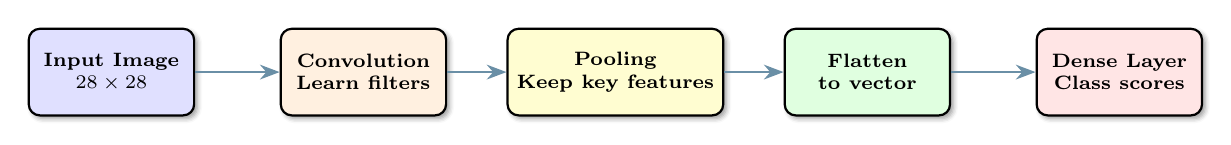
\begin{tikzpicture}[
  box/.style={rectangle, draw, thick, fill=#1, minimum width=2.1cm, minimum height=1.1cm, align=center, font=\scriptsize\bfseries, rounded corners=4pt,
    blur shadow={shadow blur steps=4, shadow xshift=0.4mm, shadow yshift=-0.4mm}},
  arr/.style={-{Stealth[length=2.5mm]}, thick, primary!65}
]
  \node[box=blue!12] (img) at (0,0) {Input Image\\$28 \times 28$};
  \node[box=orange!12] (conv) at (3.2,0) {Convolution\\Learn filters};
  \node[box=yellow!18] (pool) at (6.4,0) {Pooling\\Keep key features};
  \node[box=green!12] (flat) at (9.6,0) {Flatten\\to vector};
  \node[box=red!10] (dense) at (12.8,0) {Dense Layer\\Class scores};

  \draw[arr] (img) -- (conv);
  \draw[arr] (conv) -- (pool);
  \draw[arr] (pool) -- (flat);
  \draw[arr] (flat) -- (dense);
\end{tikzpicture}
\end{center}

\begin{itemize}[leftmargin=*]
  \item \textbf{CNNs} are strong for image tasks because nearby pixels usually belong together.
  \item \textbf{RNNs and LSTMs} are useful when order matters, such as sentences or time series.
  \item \textbf{Transformers} are now dominant in many language tasks and increasingly in vision tasks.
\end{itemize}

\subsection{Understanding Attention in One Sentence}

\begin{conceptbox}[Attention]
Attention helps a model focus on the \textbf{most relevant parts of the input} instead of treating every part as equally important. This is one reason transformers work so well in language models and modern AI systems.
\end{conceptbox}

%=============================================================
\section{A Practical Deep Learning Workflow}
%=============================================================

\begin{center}
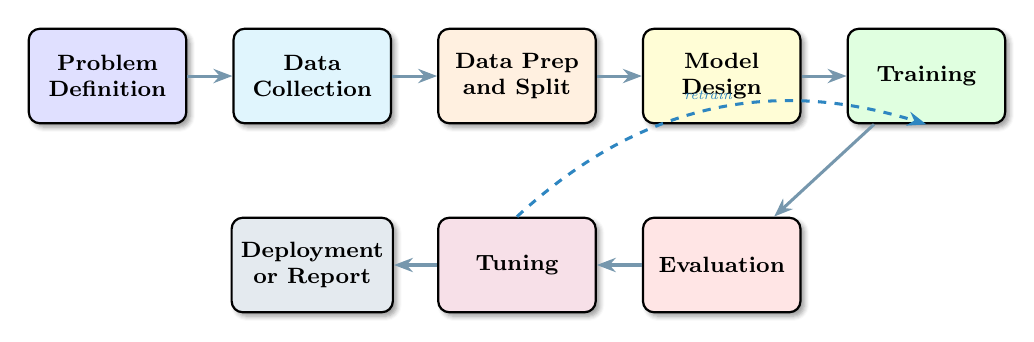
\begin{tikzpicture}[
  step/.style={rectangle, draw, thick, fill=#1, minimum width=2.0cm, minimum height=1.2cm, align=center, font=\footnotesize\bfseries, rounded corners=4pt,
    blur shadow={shadow blur steps=5, shadow xshift=0.5mm, shadow yshift=-0.5mm}},
  arr/.style={-{Stealth[length=2.4mm]}, very thick, primary!60, line width=1.1pt}
]
  \node[step=blue!12] (s1) at (0,0) {Problem\\Definition};
  \node[step=cyan!12] (s2) at (2.6,0) {Data\\Collection};
  \node[step=orange!12] (s3) at (5.2,0) {Data Prep\\and Split};
  \node[step=yellow!16] (s4) at (7.8,0) {Model\\Design};
  \node[step=green!12] (s5) at (10.4,0) {Training};
  \node[step=red!10] (s6) at (7.8,-2.4) {Evaluation};
  \node[step=purple!12] (s7) at (5.2,-2.4) {Tuning};
  \node[step=primary!12] (s8) at (2.6,-2.4) {Deployment\\or Report};

  \draw[arr] (s1) -- (s2);
  \draw[arr] (s2) -- (s3);
  \draw[arr] (s3) -- (s4);
  \draw[arr] (s4) -- (s5);
  \draw[arr] (s5) -- (s6);
  \draw[arr] (s6) -- (s7);
  \draw[arr] (s7) -- (s8);
  \draw[arr, dashed, secondary] (s7.north) to[bend left=30] node[above, font=\tiny\itshape, secondary] {retrain} (s5.south);
\end{tikzpicture}
\end{center}

\subsection{Step-by-Step View}

\begin{enumerate}[leftmargin=*]
  \item Define the task clearly: classification, regression, forecasting, or generation.
  \item Collect and clean the data.
  \item Choose how to represent the data for the model.
  \item Select a suitable architecture.
  \item Train the model and monitor loss and validation performance.
  \item Evaluate using appropriate metrics.
  \item Improve the model with tuning, regularization, or better data.
  \item Deploy the model or present findings.
\end{enumerate}

%=============================================================
\section{Easy-to-Understand Examples}
%=============================================================

\subsection{Example 1: Handwritten Digit Recognition}

\begin{examplebox}[How a CNN Reads Digits]
Suppose we want to classify images of handwritten digits from 0 to 9.
\begin{enumerate}[leftmargin=*]
  \item The input is a small grayscale image.
  \item Early CNN layers detect edges and simple curves.
  \item Later layers combine those patterns into shapes such as loops or corners.
  \item The output layer gives probabilities for classes 0, 1, 2, ..., 9.
  \item The class with the highest probability becomes the prediction.
\end{enumerate}
This example is popular because it shows how deep learning learns features automatically from images.
\end{examplebox}

\subsection{Example 2: Sentiment Analysis of Reviews}

\begin{examplebox}[Positive or Negative?]
Input text: \textit{``This mobile app is fast and easy to use.''}

Possible workflow:
\begin{itemize}[leftmargin=*]
  \item Convert words into tokens or embeddings.
  \item Use an RNN, LSTM, or Transformer to process word order and meaning.
  \item Predict whether the review is positive, negative, or neutral.
\end{itemize}
This helps students connect deep learning to real IT applications such as customer feedback analysis and chatbot improvement.
\end{examplebox}

\subsection{Example 3: Student Support Prediction}

\begin{examplebox}[A BSIT-Friendly Tabular Example]
Imagine a dataset with features such as attendance, laboratory score, quiz average, and assignment completion. A small multilayer perceptron can learn whether a student may need early academic support.

This is useful because it shows that deep learning can also work with \textbf{tabular educational data}, not only images and text.
\end{examplebox}

\subsection{A Small Keras-Style Example}

\begin{lstlisting}
from tensorflow.keras import Sequential
from tensorflow.keras.layers import Dense

model = Sequential([
    Dense(8, activation="relu", input_shape=(4,)),
    Dense(4, activation="relu"),
    Dense(1, activation="sigmoid")
])

model.compile(optimizer="adam",
              loss="binary_crossentropy",
              metrics=["accuracy"])

model.fit(X_train, y_train, epochs=20, batch_size=16)
model.evaluate(X_test, y_test)
\end{lstlisting}

\begin{conceptbox}[What This Code Shows]
The code creates a simple neural network with two hidden layers, chooses an optimizer and loss function, trains on the training set, and then evaluates performance on unseen test data.
\end{conceptbox}

%=============================================================
\section{Evaluation, Overfitting, and Improvement}
%=============================================================

\subsection{Useful Evaluation Metrics}

\begin{itemize}[leftmargin=*]
  \item \textbf{Accuracy:} Overall percentage of correct predictions.
  \item \textbf{Precision:} When the model predicts positive, how often is it correct?
  \item \textbf{Recall:} Of all real positives, how many did the model find?
  \item \textbf{F1-score:} Balance between precision and recall.
  \item \textbf{MAE / MSE / RMSE:} Common for regression problems.
\end{itemize}

\subsection{Overfitting vs. Underfitting}

\begin{center}
\begin{tabular}{@{}p{6.4cm}p{6.4cm}@{}}
\toprule
\textbf{Underfitting} & \textbf{Overfitting} \\
\midrule
Model is too simple & Model memorizes training data \\
Poor on training data and test data & Very good on training data, weak on new data \\
Needs more model capacity or better features & Needs regularization, more data, or simpler design \\
\bottomrule
\end{tabular}
\end{center}

\subsection{How to Reduce Overfitting}

\begin{itemize}[leftmargin=*]
  \item Use more training data if available.
  \item Apply \textbf{dropout} so some neurons are randomly ignored during training.
  \item Use \textbf{early stopping} to stop training when validation performance stops improving.
  \item Add \textbf{data augmentation} for image tasks.
  \item Reduce the model size if it is unnecessarily large.
\end{itemize}

\subsection{Common Problems and Practical Remedies}

\rowcolors{2}{white}{defbg}
\begin{longtable}{@{}p{3.6cm}p{4.2cm}p{5.3cm}@{}}
\toprule
\rowcolor{primary!15}
\textbf{Problem} & \textbf{Typical Symptom} & \textbf{Practical Remedy} \\
\midrule
\endhead
Overfitting & Validation accuracy drops while training accuracy keeps rising & Dropout, early stopping, more data, smaller model \\
\addlinespace
Underfitting & Both training and validation performance stay low & More layers, more epochs, better features, better tuning \\
\addlinespace
Data shortage & Model performance is unstable & Gather more data, augment data, use transfer learning \\
\addlinespace
Class imbalance & Rare cases are missed & Resampling, class weights, better metrics than accuracy alone \\
\addlinespace
High compute cost & Training takes too long & Use smaller model, smaller batch, GPU, or pretrained models \\
\bottomrule
\end{longtable}

%=============================================================
\section{Deep Learning vs. Traditional Machine Learning}
%=============================================================

\begin{center}
\begin{tabular}{@{}p{3.6cm}p{4.3cm}p{4.6cm}@{}}
\toprule
\textbf{Aspect} & \textbf{Traditional ML} & \textbf{Deep Learning} \\
\midrule
Feature engineering & Often manual and important & Often learned automatically \\
Data requirement & Can work well on smaller datasets & Usually benefits from large datasets \\
Interpretability & Often easier to explain & Often harder to interpret \\
Computing need & Usually lower & Usually higher \\
Best known strengths & Tabular business data, interpretable models & Images, speech, text, complex patterns \\
\bottomrule
\end{tabular}
\end{center}

\begin{conceptbox}[Practical Advice for Students]
If your dataset is small and highly structured, start with traditional machine learning. If your data is complex, unstructured, and large, deep learning becomes much more attractive.
\end{conceptbox}

%=============================================================
\section{Best Practices Checklist}
%=============================================================

\begin{itemize}[leftmargin=*]
  \item Clearly define the target variable and success metric.
  \item Understand the data before choosing the model.
  \item Start with a simple baseline before building a deeper network.
  \item Split data correctly into training, validation, and test sets.
  \item Monitor both training and validation performance.
  \item Record hyperparameters and results for each experiment.
  \item Use regularization methods when overfitting appears.
  \item Prefer pretrained models when data or time is limited.
  \item Evaluate the model on unseen data before reporting success.
  \item Consider fairness, privacy, and bias in the dataset.
\end{itemize}

%=============================================================
\section{Mini Case Study for BSIT Data Science}
%=============================================================

\begin{definitionbox}[Scenario]
A BSIT department wants to identify students who may need extra academic support early in the semester. The available data includes attendance, laboratory activities, quiz averages, assignment completion, and previous subject performance.
\end{definitionbox}

\textbf{Possible workflow:}
\begin{enumerate}[leftmargin=*]
  \item Define the target as \textit{needs support} or \textit{does not need support}.
  \item Clean missing records and encode the data.
  \item Split the dataset into training, validation, and test sets.
  \item Train a small MLP model.
  \item Compare it with logistic regression as a baseline.
  \item Evaluate using accuracy, precision, and recall.
  \item Use the final model carefully as a decision-support tool, not as an automatic final judgment.
\end{enumerate}

\begin{alertbox}[Responsible Use]
Predictions about students should support teachers and advisers, not replace human judgment. Educational models can be useful, but they must be used ethically and checked for bias.
\end{alertbox}

%=============================================================
\section{Summary}
%=============================================================

\begin{itemize}[leftmargin=*]
  \item Deep learning is a powerful subset of machine learning built from many connected neurons.
  \item The basic flow is: input data $\rightarrow$ forward pass $\rightarrow$ loss $\rightarrow$ backpropagation $\rightarrow$ weight update.
  \item Different architectures suit different data types: MLP for tabular data, CNN for images, RNN/LSTM for sequences, and Transformers for attention-based modeling.
  \item Good data preparation, proper evaluation, and regularization are essential.
  \item For BSIT Data Science students, deep learning is most useful when the problem involves complex patterns in large or unstructured data.
\end{itemize}

%=============================================================
\section{Review Questions}
%=============================================================

\begin{enumerate}[leftmargin=*]
  \item What is the difference between artificial intelligence, machine learning, and deep learning?
  \item What does a neuron do inside a neural network?
  \item Why do neural networks need activation functions?
  \item In simple words, what is the purpose of backpropagation?
  \item What is the difference between a parameter and a hyperparameter?
  \item Why do we use separate validation and test sets?
  \item Which architecture would you choose for image classification, and why?
  \item What is overfitting, and how can it be reduced?
  \item Why might a traditional machine learning model still be better than deep learning in some projects?
  \item How can deep learning be applied responsibly in an educational setting?
\end{enumerate}

\end{document}